%-----------------------------------------------------------------------------
%
%               Template for sigplanconf LaTeX Class
%
% Name:         sigplanconf-template.tex
%
% Purpose:      A template for sigplanconf.cls, which is a LaTeX 2e class
%               file for SIGPLAN conference proceedings.
%
% Guide:        Refer to "Author's Guide to the ACM SIGPLAN Class,"
%               sigplanconf-guide.pdf
%
% Author:       Paul C. Anagnostopoulos
%               Windfall Software
%               978 371-2316
%               paul@windfall.com
%
% Created:      15 February 2005
%
%-----------------------------------------------------------------------------


\documentclass[11pt]{sigplanconf}

% The following \documentclass options may be useful:

% preprint      Remove this option only once the paper is in final form.
% 10pt          To set in 10-point type instead of 9-point.
% 11pt          To set in 11-point type instead of 9-point.
% authoryear    To obtain author/year citation style instead of numeric.

\usepackage{amsmath}

\usepackage{graphicx}
\graphicspath{ {images/} } % Path to images folder

\begin{document}

\special{papersize=8.5in,11in}
\setlength{\pdfpageheight}{\paperheight}
\setlength{\pdfpagewidth}{\paperwidth}

\conferenceinfo{CONF '14}{September 29, 2014, 2014, Golden, CO, USA} 
\copyrightyear{2014} 
\copyrightdata{978-1-nnnn-nnnn-n/yy/mm} 
\doi{nnnnnnn.nnnnnnn}

% Uncomment one of the following two, if you are not going for the 
% traditional copyright transfer agreement.

%\exclusivelicense                % ACM gets exclusive license to publish, 
                                  % you retain copyright

%\permissiontopublish             % ACM gets nonexclusive license to publish
                                  % (paid open-access papers, 
                                  % short abstracts)

\titlebanner{banner above paper title}        % These are ignored unless
\preprintfooter{short description of paper}   % 'preprint' option specified.

\title{GPU-Based Parallel Finite State Machines}

\authorinfo{Kameron W. Kincade\and Ryan P. Langewisch}
           {Colorado School of Mines}
           {kkincade@mines.edu | rlangewi@mines.edu}

\maketitle

%\begin{abstract}
%Abstract goes here.
%\end{abstract}

% general terms are not compulsory anymore, 
% you may leave them out
\terms
finite state machines, GPU, parallelization

\section{Introduction}
 
A finite-state machine is used to represent an object that can exist in a limited number of states and that can change state based on a number of well-defined rules (Figure 1). Each finite-state machine is responsible for processing various inputs (each usually represented as a string of characters) and determining if these inputs satisfy the machine's acceptance criteria, represented by ending in one of the machine's final states. To operate on an input string, the finite-state machine begins with the start state (A in Figure 1) and processes each character one after another. The state machine's transition rules, along with the input character, dictate the next location to move to. An acceptance state (D) is commonly indicated by a double circle and represents a valid input solution that satisfies the finite-state machine's criteria.

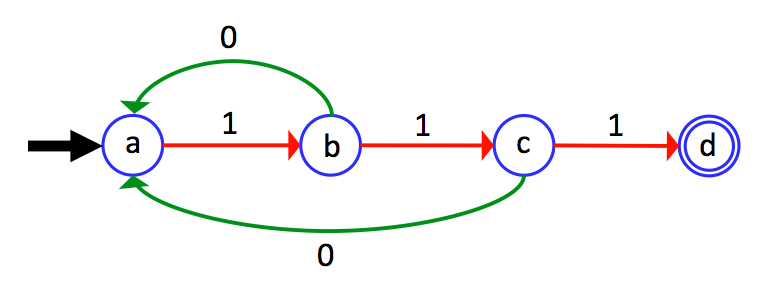
\includegraphics[width=\linewidth]{fsm_diagram.png}

Finite-state machines are embedded in many different types of applications, including web application computations such as lexing, parsing, translations, and media encoding/decoding. With the recent emphasis on mobile, handheld devices, the need for a computationally efficient implementation of finite-state machines is becoming more important. Parallelization is one of the obvious ways to speed up the execution of a program. However, the exclusively sequential execution of finite-state machines makes them difficult to parallelize. In this paper, we will describe some of the relevant work in the area of parallelizing finite-state machines, describe our goal and implementation progress, and then detail optimizations that we have considered adding as well as future work that could be done to extend the scope of our implementation. 
 
\section{Related Work}
 
The objective of parallelizing a finite-state machine is a relatively unexplored topic in computer science. To our knowledge, there are only two main publications regarding methods to parallelize finite-state machines: \textit{Data Parallel Finite-State Machines} [1] and \textit{Challenging the ``Embarrassingly Sequential'': Parallelizing Finite State Machine-Based Computations through Principled Speculation} [2]. The two prior publications utilize noticeably different techniques in attempts to adapt finite-state machines to work in a non-serial implementation. These two different methodologies will be described within this section.

The paper \textit{Data Parallel Finite-State Machines} [1] presents a parallel algorithm which performs finite-state machine computations while utilizing different kinds of data parallelism across multiple processors, as well as within a single processor. The key concept of the algorithm involves splitting the input string into distinct chunks (e.g. sub-computations on the finite-state machine) and processing the distinct chunks simultaneously. The problem with this approach is knowing the start states for each of the distinct sub-computations, as each chunk is directly influenced by the end state of the sub-computation previous to it. The authors of the paper address this data dependency by using an enumerative approach. The enumerative approach involves evaluating the sub-computation using all possible start states (i.e. enumerating over all possible start states). Once the first computation finishes, the algorithm selects the version of the enumerative computation that started from the correct start state. This process can be generalized by splitting the input string into any number of distinct chunks, with all but the first being processed in parallel.

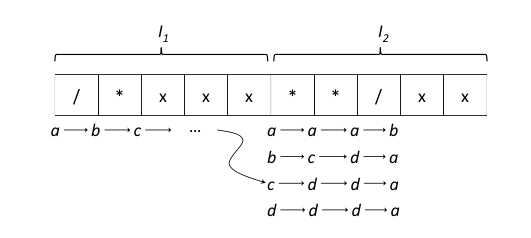
\includegraphics[width=\linewidth]{enumerative_overview.png}

The main disadvantage of the enumerative approach is the amount of wasted computations being performed. This overhead is directly proportional to the amount of states within the finite-state machine. For example, a finite-state machine with n states will perform n times more computations than its corresponding serial counterpart. The paper describes different optimizations to make the enumerative computation more efficient. The main optimization relies on the assessment that many of the different enumerations of a given sub-computation converge to the same state on the same input symbol. Through dynamically utilizing this convergence, the overhead becomes proportional to the number of active states, which the authors describe as states that do not arrive from redundant (convergent) computations. This, along with other noted optimizations, offers an average of a three times speedup in exchange for the added overhead.

The other paper \textit{Challenging the ``Embarrassingly Sequential'': Parallelizing Finite State Machine-Based Computations through Principled Speculation} [2] suggests a different way of parallelizing a finite-state machine. Rather than running an enumerative computation, the authors suggest a lookback method. While still splitting the input string into multiple sub-computations, the lookback methodology attempts to provide some amount of context, using a number of ending symbols (i.e. a suffix), to help speculate the start state of a given sub-computation. The context does not necessarily provide us with the correct start state, but it can help eliminate states in which it is impossible for a given sub-computation to start with. Although this is not a new concept, the authors provide speculate as to why this approach has been rather unsuccessful in prior attempts.

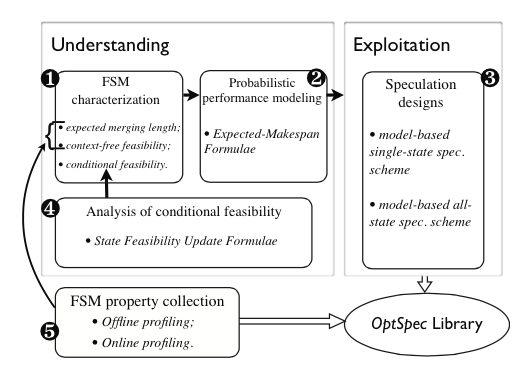
\includegraphics[width=\linewidth]{lookback_profiling_overview.png}

The authors suggest factors, such as the number of symbols used in the lookback and the state used to begin the lookback, as just a few of the ways to possibly improve performance. They describe a collection of these factors as a speculation scheme. The main principle of their approach involves an element of profiling, by characterizing an finite-state machine and matching its properties and input to a speculation scheme that minimizes the expected make-span, which is the mean of all execution times for multiple, different length inputs. By matching a speculation scheme to a particular FSM, the concept of lookback can be utilized more efficiently, thus leading to an overall performance optimization for a given FSM and a given input string.

\section{Project Goal}

In the case of both of the fore-mentioned papers, which are the most recent and relevant work on this topic, finite-state machines were implemented in parallel, but not using GPU. It is this fact that leads us to the primary goal for our project: \textbf{Our goal is to implement deterministic finite state machines on GPU}. Additionally, we are going to focus on developing an implementation that applies all optimizations at run-time, with no prerequisite profiling. Our approach will consist of initially just getting an implementation working on GPU without any optimization, and then we will attempt to add in modular layers of optimization such as the techniques discussed in the above papers. This goal is challenging for many of the same reasons that finite-state machines are difficult to implement on CPU: the process of a finite-state machine is as sequential as a process can possibly be. Every single instruction is data dependent on the previous instruction. For this reason, it becomes an interesting problem to try and parallelize, and requires a different approach than most program optimizations using parallelization. Further interest is added to the topic due to the fact that no research has been done specifically with finite-state machines on GPU, making any progress or working implementation a contribution to the field. 

\section{Implementation}

In order to fully understand how to implement a parallelized version of a finite-state machine, we decided that our first step should be to decide upon the tools and hardware that should be used. As far as hardware is concerned, we currently have a good range of GPUs at our disposal. This range includes a Macbook Pro using a sixteen core NVIDIA GeForce 9400M, a Mac Pro equipped with an NVIDIA GeForce GTX 650 Ti Boost, and a GPU server provided by the Colorado School of Mines (specs currently unknown). Some detailed specs of the GPUs are given in the table below.

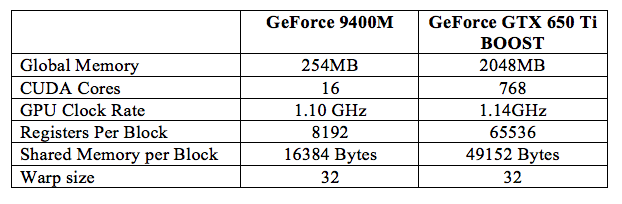
\includegraphics[width=\linewidth]{gpu_specs.png}

Beyond hardware, the CUDA (Compute Unified Device Architecture) programming language, which is an extension of the C/C++ language developed by NVIDIA for parallel programming, was recommended as one of the easier parallel frameworks to pick up quickly. Due to the limited amount of time, a prior knowledge of the C++ language, and CUDA's compatibility with our NVIDIA GPUs, we concluded that this was the best choice of language. As a result, a large portion of our time was spent learning and understanding exactly how CUDA works. This included understanding CUDA syntax for declaring and calling kernels, how to correctly allocate and access both global and local memory, and how to collect results from each thread once it has completed its unit of work. Obviously understanding CUDA will continue to be a work in progress, but we now have a solid grasp on the framework and its underlying properties.

After deciding on a language and compatible hardware, our next step was constructing a simple, serial implementation of a finite-state machine to help us determine the the best way to represent the machine in a data structure. Our first approach was representing the finite-state machine through the use of two C++ maps, entitled fsm and stateTransitions. The fsm map is responsible for mapping a state to its corresponding transition table (i.e. stateTransitions), which is in turn responsible for mapping an input character to the next state of the finite-state machine. Therefore, determining the next state of the finite-state machine is as simple as accessing fsm[currentState][inputSymbol]. 

With a working serial version implemented, our next goal was to implement a version of a finite-state machine that would run serially on each thread through the use of a CUDA kernel. In essence, each thread would run the exact same input on the exact same finite-state machine in order to solidify our understanding of how a CUDA application works. This seemed like a straightforward process, but the quick realization that CUDA has no support for the C++ stl library made us rethink the whole structure of our finite-state machine. Without the use of maps, we were forced to implement a version that utilized arrays to represent our finite-state machine within memory. This new representation was structured using a two dimensional array. Each row in the array represents a state in the finite-state machine, and each column corresponds to an input symbol. The resulting elements of the array represent the resulting states given a start state and an input symbol.

Our newly devised two-dimensional array representing our finite-state machine needed to be stored in global memory, in order for every thread to have access to it. Since all threads had access to the finite-state machine, each thread required only a start state and an input string in order to run the finite-state machine and compute the corresponding end state. With a simplified CUDA version of a finite-state machine implemented, we are now in the position to begin optimizations.

\section{Optimizations}

At this point in our implementation, there is no benefit from running the finite-state machine on a GPU (it is currently being ran serially), and the additional overhead of the parallel architecture actually makes it even less desirable. In order to make the GPU implementation notable at all, we need to employ strategies to specifically utilize the additional cores that are available within GPU to maximize the parallelization. 

Our first planned optimization it to implement a simple enumerative approach. This is going to be the primary technique for actually branching the problem into parallel executions. The basic idea is that that the input string is split into a number of equal chunks determined by some predefined constant value. The first chunk, which represents the beginning of the input string, will be run on the first thread, and its result is guaranteed to be useful since it would have been the first portion of the string to be executed even if the finite-state machine was run serially. But instead of waiting for the first chunk of the string to complete to start the next chunk, we are going to run the second chunk in parallel using a guess for what the initial state should be. When the first chunk finishes, the host program will use the actual result state to determine which of the ``prediction chunks'' was computing from the matching start state. This obviously leads to a lot of computed results that are left unused, but that is an advantage that comes with using GPU. Since so many threads can be run independently, we might as well be computing something on each thread rather than leaving a number of them idle. 

This will then become an iterative process: the host device first deploys the current chunk onto a GPU thread. It then deploys a number of prediction chunks that will then run in parallel with the current chunk. Once all threads complete, the host device will piece together the results based on the current chunk?s final state, and determine the new current chunk. This is repeated until the entire input string is exhausted. While the core idea of this optimization technique is fairly straightforward, there are a lot of parameters that can be tweaked to affect its impact on performance. For example, the chunk size is going to have an impact on the ratio of running time on the CUDA device to the amount of overhead that the host device needs to spend deploying new threads. In addition, there are some decisions to be made about which prediction chunks should be used. 

One approach is to apply a breadth-first search to determine which chunks are deployed first. This means the second chunk is going to be deployed along with every possible start state before any threads are deployed with the third chunk of the input string. This is useful because if all the possible start states are considered for the the second chunk, the correct state is guaranteed to have been evaluated by the time the first chunk finishes. The other extreme is if we apply a depth-first search for our chunk selection strategy. This would mean that we only consider one start state for every chunk in the string, allowing many sequential chunks in the string to be run at the same time. This approach would actually be extremely ineffective, because if any of the single guessed states for a given chunk is wrong, all following chunk computations are useless because we need to recompute the chunk that was miscalculated. In other words, a strictly depth-first approach requires us to exactly guess correctly to reap any computational benefit. But a hybrid approach between breadth-first and depth-first could prove to be effective if we can find a balance between maintaining a high probability of having the next chunk result precomputed, while still having the chance of multiple chunk completion within a single kernel call.

This leads us to the topic of attempting to trim down the start states that are considered for each chunk. If we can determine that a certain start state is unreachable for that specific chunk, we can exclude it, allowing us to maximize the effectiveness of the chunks that are run during each iteration. This can be approached using the lookback technique described in one of the papers of previous work. Instead of simply running an instance of the chunk for every start state, the algorithm will also look at a certain number of input symbols before the chunk in attempt to eliminate some start states from the search space. In the paper that implemented the lookback technique, there was significant profiling that was applied before the actual parallel finite-state machine implementation was run. As stated in our goal for the project, we are trying to focus on optimizations that can be applied at runtime, without any profiling in advance. This is going to make implementing lookback slightly more challenging, as any data about what states are possible needs to be generated as part of the overall execution time.

One approach to this might be to apply some sort of dynamic learning algorithm that gathers more information about how to filter states with each iteration of chunks that is run by the finite-state machine. At the very least, a very simple implementation could be added that at least rules out states based on a small lookback. For example, if the input symbol before the chunk is a zero, we can immediately rule out any state that does not have a transition of zero moving into it. This can be applied a variable amount of steps back in the input string, which introduces another parameter to be considered. The larger the lookback, the more states that can be eliminated from the search space, freeing threads to run computations that have more potential of use. The drawback is that the overhead on the host device also increases with a larger lookback. It is another balancing act to find the most effective strategy, and the ``right answer'' is dependent on a large amount of factors including, but not limited to: the number of states in the finite-state machine, the number of different input symbols, and the current chunking strategy that is being used (the balance between breadth-first and depth-first selection of prediction chunks).

As mentioned before, our current implementation places the finite-state machine data structure into the global memory of CUDA so that it can be accessed by all of the individual threads that are running. This works fine as a preliminary approach, but global memory happens to be the slowest memory strategy in CUDA. Another optimization that could be made is to transition the finite-state machine into shared memory to allow for more efficient data accesses. The problem presented by finite-state machines has the advantage of not needing to write any data to shared memory; the finite-state machine remains constant throughout the entire run. This means that we don?t need to worry about any problems caused by data racing or other dependencies in shared memory. That said, memory accesses to the finite-state machine make up the majority of the computation that happens within the CUDA kernel, and therefore any optimization to the data accesses will have its benefit multiplied significantly in the context of the entire execution.
	
\section{Future Work}

For this project, we intentionally narrowed the problem scope to make it more manageable. One of the restrictions that we set for ourselves was to avoid any pre-run profiling. There is nothing about our implementation that prevents this strategy from being added, and one future extension would be to create a profiling algorithm that improves the accuracy of the decisions that the program needs to make at runtime. The scope of the problem could also be expanded to include non-deterministic finite-state machines. This would likely require a major reworking of the thread-chunking algorithm, but could allow the work be applied to other applications. Similarly, there may be different optimizations that can be made based on properties of the finite-state machine such as number of states, density of edges, and number of cycles. Due to the fact that finite-state machines can be defined with such a wide variance in properties, there are a lot of tests and specific approaches that could be applied to address different applications. Our work should lay some of the groundwork for these optimizations to be explored.


%\appendix
%\section{Appendix Title}

%This is the text of the appendix, if you %need one.

%\acks

%Acknowledgments, if needed.

% We recommend abbrvnat bibliography style.

%\bibliographystyle{abbrvnat}

% The bibliography should be embedded for final submission.

%\begin{thebibliography}{}
%\softraggedright

%\bibitem[Smith et~al.(2009)Smith, Jones]%{smith02}
%P. Q. Smith, and X. Y. Jones. %...reference text...

%\end{thebibliography}


\end{document}

%                       Revision History
%                       -------- -------
%  Date         Person  Ver.    Change
%  ----         ------  ----    ------

%  2013.06.29   TU      0.1--4  comments on permission/copyright notices